%!TEX program = pdflatex

% UQ Gemini theme
% See: https://github.com/alfurka/gemini-uq
% Forked from
% https://rev.cs.uchicago.edu/k4rtik/gemini-uccs
% which is forked from
% https://github.com/anishathalye/gemini


\documentclass[noamssymb]{beamer}

% ====================
% Packages
% ====================

%\usepackage[T1]{fontenc}
\usepackage{lmodern}
\usepackage[size=custom,width=90,height=130,scale=1.0]{beamerposter}
\usetheme{gemini}
\usecolortheme{uchicago}
\usepackage{graphicx}
\usepackage{booktabs}
\usepackage{tikz}
\usepackage{pgfplots}
\usepackage{newtxtext}
%\usepackage[default]{raleway}
\usepackage[sfdefault]{carlito}
\usefonttheme{professionalfonts}
\usepackage[subscriptcorrection,nofontinfo]{mtpro2}
\usepackage{physics}


\usepackage{hyperref}% add hypertext capabilities
\usepackage{xcolor}
\hypersetup{
	colorlinks   = true, %Colours links instead of ugly boxes
	urlcolor     = blue, %Colour for external hyperlinks
	linkcolor    = blue, %Colour of internal links
	citecolor   = red %Colour of citations
}
\pgfplotsset{compat=1.17}

% ====================
% Lengths
% ====================

% If you have N columns, choose \sepwidth and \colwidth such that
% (N+1)*\sepwidth + N*\colwidth = \paperwidth
\newlength{\sepwidth}
\newlength{\colwidth}
\setlength{\sepwidth}{0.01\paperwidth}
\setlength{\colwidth}{0.32\paperwidth}

\newcommand{\separatorcolumn}{\begin{column}{\sepwidth}\end{column}}

% ====================
% Title
% ====================

\title{Numerical Relativity Studies of Spin-Configured Binary Black Hole}

\author{Dongchan Kim \inst{1} \and Gungwon Kang \inst{1}}

\institute[shortinst]{\inst{1} Department of Physics, Chung-Ang University}

% ====================
% Footer (optional)
% ====================

\footercontent{
  2023. 11. 13 \hfill
  2023 CAU Physics Academic \hfill
  krq3268@cau.ac.kr}
% (can be left out to remove footer)

% ====================
% Logo (optional)
% ====================

% use this to include logos on the left and/or right side of the header:
% \logoright{\includegraphics[height=7cm]{logo1.pdf}}
% \logoleft{\includegraphics[height=7cm]{logo2.pdf}}

% ====================
% Body
% ====================

\begin{document}
\addtobeamertemplate{headline}{}
{
    \begin{tikzpicture}[remember picture,overlay]
      \node [anchor=north west, inner sep=3cm] at ([xshift=0.0cm,yshift=2.0cm]current page.north west)
      {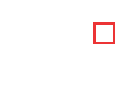
\includegraphics[height=6.6cm]{logos/blue_emblem.pdf}}; % also try shield-white.eps
      \node [anchor=north east, inner sep=3cm] at ([xshift=0.0cm,yshift=2.5cm]current page.north east)
      {
\includegraphics[height=8.0cm]{logos/white.pdf}};
    \end{tikzpicture}
}

\begin{frame}[t]
\begin{columns}[t]
\separatorcolumn

\begin{column}{\colwidth}

  \begin{block}{Abstract}

    We present a numerical relativistic study of spinning binary black holes. We investigate their dynamics with respect to black hole spins by simulating two cases. We compare how their dynamics are affected by spin. We find that the case where the spins are aligned with the orbital angular momentum forms more orbits and emits more energy and angular momentum compared to the case where the spins are anti-aligned. We calculate energy and angular momentum using two different methods and confirm their validity.

  \end{block}
  
  \begin{block}{Introduction}
  	
  	The successful numerical calculations of the motion of binary black hole systems and the resulting gravitational waveforms have been a major focus since the emergence of numerical relativity. Gravitational waves emitted from binary black hole systems generate the strongest observable gravitational signals. To actually observe them, accurate gravitational waveforms are essential. Following the successful calculations in 2005 by \cite{Campanelli:2005dd, Baker:2005vv, Pretorius:2005gq}, where black holes with no spin started from quasi-circular orbits and merged, emitting gravitational waves, research continued to investigate the behavior of the system concerning various physical quantities, such as the masses, spins, and eccentricities of the two black holes.
  	
  	In this study, we present the time to merger, gravitational waveforms, emitted energy, and angular momentum, depending on whether two black holes of equal mass are in a aligned or antialigned with the orbital angular momentum. The next section outlines how we constructed the initial data and the gauge conditions and evolution methods used. We then present the results for different spin orientations.
  	
  \end{block}
  
  \begin{block}{Grid Setup}
  	
  	The simulation was conducted using the \textsc{Einstein Toolkit}\cite{EinsteinToolkit:2023_05}. In each simulation, the initial total ADM mass was scaled to $M$, and the geometric units were adopted with $c=G=1$.
  	
  	The two black holes moved in the $xy$ plane, utilizing $xy$ plane symmetry to conserve computational resources. A multipatch coordinate system\cite{Pollney:2009yz} was employed as the coordinate system. Adaptive mesh refinement was implemented through \textsc{Carpet}\cite{CarpetCode:web} centered around each black hole puncture. The base grid spacing was $0.9172M$, with the finest grid spacing being $0.0036M$.
  	
  \end{block}
  
  \begin{block}{Initial data}
  	
  	To observe the effects of spin, it is essential to determine the appropriate separation, momentum, and spin using post-Newtonian theory. We based our values on the physical quantities presented in \cite{Campanelli:2006uy}. 
  	
  	\begin{table}
  		\centering
  		\begin{tabular}{c c c}
  			\toprule
  			\textbf{} & \textbf{Aligned} & \textbf{Antialigned}\\
  			\midrule
  			$x/M$ & 3.0595 & 3.465 \\
  			$P/M$ & 0.1291 & 0.1382 \\
  			$S/M^2$ & +0.1939 & -0.1924 \\
  			$J/M^2$ & 1.1778 & 0.5729 \\
  			$L/M^2$ & 0.7900 & 0.9577 \\
  			$\mathcal{M}/M$ & 0.3344 & 0.3344\\
  			\bottomrule
  		\end{tabular}
  		\caption{Initial data for black hole binaries. The holes have puncture locations $(\pm x, 0, 0)$, linear momenta $(0, \pm P, 0)$, and spin $(0, 0, S)$.}
  	\end{table}
  	
  	\begin{figure}
  		\centering
  		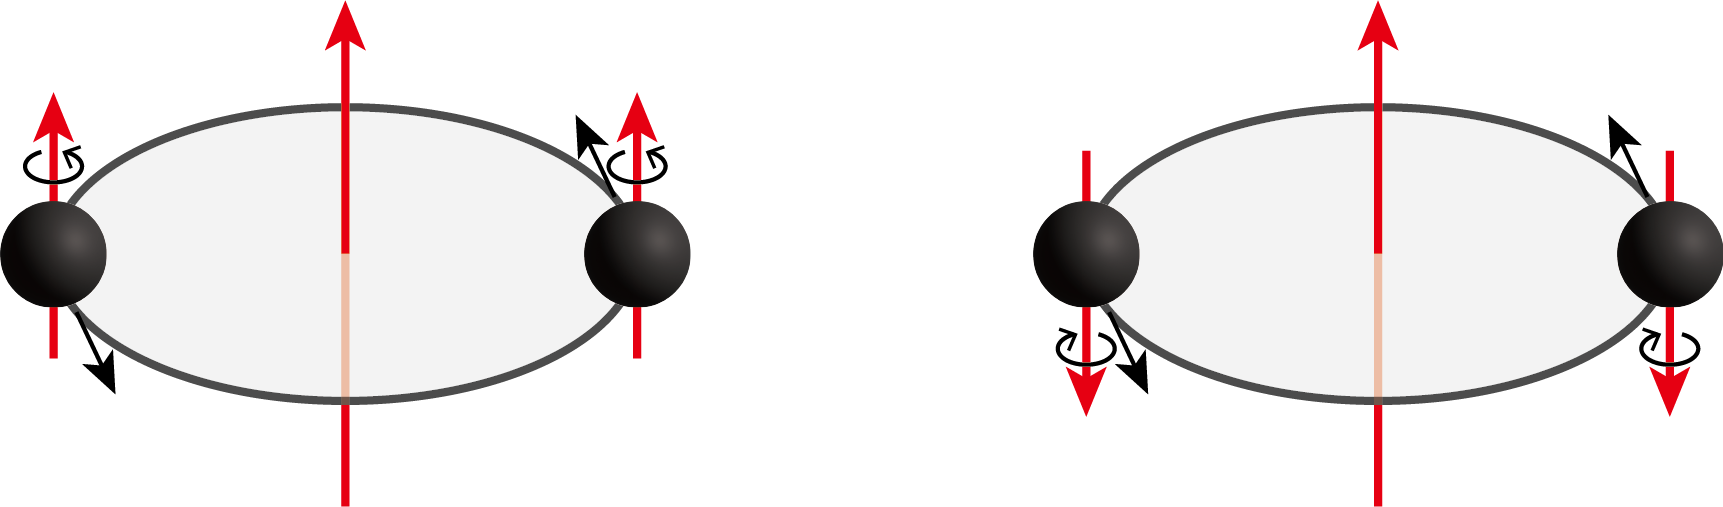
\includegraphics[width=0.8\columnwidth]{img/intro}
  		\caption{\label{fig:intro}The orientation of each black hole's spin and orbital angular momentum. Left shows the spin aligned case and right shows the spin antialigned case.}
  	\end{figure}
  	
  	Based on the determined physical quantities, we need to establish the metric and extrinsic curvature. This process is carried out by \textsc{TwoPunctures} \cite{Ansorg:2004ds}, which operates under the following assumptions:
  	\begin{itemize}
  		\item Conformal flatness: $\bar{\gamma}_{ij} = \eta_{ij}$.
  		\item Transverse part to vanish: $\bar{A}_\mathrm{TT}^{ij} = 0$.
  		\item Maximal slicing: $K=0$.
  	\end{itemize}
  	In this assumptions, the momentum constraint in Cartesian coordinates becomes:
  	\begin{equation}
  		\partial^j \partial_j W^i + \frac{1}{3}\partial^i\partial_j W^j = 0.
  	\end{equation}
  	This equation is linear, allowing us to construct multiple black hole solutions as a sum of solutions for individual black holes.
  	
  	For the Hamiltonian constraint, under the same assumptions, it becomes:
  	\begin{equation}
  		\bar{D}^2\psi + \frac{1}{8}\psi^{-7}\bar{A}^\mathrm{L}_{ij}\bar{A}^{ij}_\mathrm{L} = 0.
  	\end{equation}
  	The \textsc{TwoPunctures} thorn solves the above equations using a single-domain spectral method.
  	
  	
  \end{block}

  \begin{block}{Gauge Condition}

    We adopt the 1+log slicing with advection term is given by
    \begin{eqnarray}
    	\label{eq:logadv}
    	\partial_t \alpha = -2\alpha K + \beta^i \partial_i \alpha,
    \end{eqnarray}
    and the hyperbolic gamma driver condition for the shift with advection term is defined as
    \begin{eqnarray}
    	\label{eq:betaadv}
    	\partial_t \beta^i = \frac{3}{4}B^i + \beta^j\partial_j \beta^i,
    \end{eqnarray}
    \begin{eqnarray}
    	\label{eq:Badv}
    	\partial_t B^i = \partial_t \bar{\Gamma}^i -B^i + \beta^j \partial_j B^i,
    \end{eqnarray}
    which is typically employed in the moving puncture method \cite{Campanelli:2005dd, Alcubierre:2002kk}. 
    
    We used the \texttt{twopunctures-averaged} initial lapse, which is given by
    \begin{eqnarray}
    	\alpha &=& \frac{1}{2}(1 + \alpha'),
    \end{eqnarray}
    where
    \begin{eqnarray}
    	\alpha' &=& \frac{1 - \frac{\mathcal{M}_+}{2r_+} - \frac{\mathcal{M}_-}{2r_-}}{1 + \frac{\mathcal{M}_+}{2r_+} + \frac{\mathcal{M}_-}{2r_-}},
    \end{eqnarray}
    ensuring that the lapse satisfies $0 \le \alpha \le 1$.

  \end{block}

%  \begin{alertblock}{A highlighted block}
%
%    This block catches your eye, so \textbf{important stuff} should probably go
%    here.
%
%    Curabitur eu libero vehicula, cursus est fringilla, luctus est. Morbi
%    consectetur mauris quam, at finibus elit auctor ac. Aliquam erat volutpat.
%    Aenean at nisl ut ex ullamcorper eleifend et eu augue. Aenean quis velit
%    tristique odio convallis ultrices a ac odio.
%
%    \begin{itemize}
%      \item \textbf{Fusce dapibus tellus} vel tellus semper finibus. In
%        consequat, nibh sed mattis luctus, augue diam fermentum lectus.
%      \item \textbf{In euismod erat metus} non ex. Vestibulum luctus augue in
%        mi condimentum, at sollicitudin lorem viverra.
%      \item \textbf{Suspendisse vulputate} mauris vel placerat consectetur.
%        Mauris semper, purus ac hendrerit molestie, elit mi dignissim odio, in
%        suscipit felis sapien vel ex.
%    \end{itemize}
%
%    Aenean tincidunt risus eros, at gravida lorem sagittis vel. Vestibulum ante
%    ipsum primis in faucibus orci luctus et ultrices posuere cubilia Curae.
%
%  \end{alertblock}

\end{column}

\separatorcolumn

\begin{column}{\colwidth}

  \begin{block}{Evolution}
  	
  	The 3+1 ADM evolution equations are given as:
  	\begin{equation}
  		(\partial_t - \mathcal{L}_\beta)\gamma_{ij} = -2\alpha K_{ij},
  	\end{equation}
  	\begin{eqnarray}
  		(\partial_t - \mathcal{L}_\beta)K_{ij} &=& -D_i D_j \alpha + \alpha (R_{ij} + KK_{ij}-2K_{ik}K^k{}_{j}) +4\pi \alpha M_{ij},
  	\end{eqnarray}
  	
  	However, this set of partial differential equations is only weakly hyperbolic and is therefore not suitable for stable numerical evolution. To address this, we adopt the BSSN (\textit{Baumgarte-Shapiro-Shibata-Nakmura}) formulation \cite{Nakamura:1987,  Shibata:1995we, Baumgarte:1998te}.
  	
  	In the BSSN formulation, the spatial metric $\gamma_{ij}$ is decomposed into a conformally related metric, with $\det (\bar{\gamma}_{ij}) = 1$. The extrinsic curvature is also decomposed into its trace and traceless parts, and we conformally transform the traceless part as follows:
  	\begin{equation}
  		K_{ij} = e^{4\phi}\tilde{A}_{ij} + \frac{1}{3}\gamma_{ij}K.
  	\end{equation}
  	We then promote the following variables to evolution variables:
  	\begin{equation}
  		\phi = \ln \psi = \frac{1}{12}\ln \gamma,
  	\end{equation}
  	as well as the conformal connection functions:
  	\begin{equation}
  		\bar{\Gamma}^i = \bar{\gamma}^{jk}\bar{\Gamma}^i{}_{jk} = -\partial_j \bar{\gamma}^{ij}.
  	\end{equation}
  	The evolution equation for $\gamma_{ij}$ splits into two equations:
  	\begin{equation}
  		\partial_t \phi = - \frac{1}{6}\alpha K + \beta^i \partial_i \phi + \frac{1}{6}\partial_i \beta^i,
  	\end{equation}
  	\begin{eqnarray}
  		\label{eq:bssn_gamma}
  		\partial_t \bar{\gamma}_{ij} &=& -2\alpha \tilde{A}_{ij} + \beta^k \partial_k \bar{\gamma}_{ij}  +\bar{\gamma}_{ik}\partial_j \beta^k + \bar{\gamma}_{jk}\partial_i \beta^k - \frac{2}{3}\bar{\gamma}_{ij}\partial_k\beta^k.
  	\end{eqnarray}
  	The evolution equation for $K_{ij}$ also splits into two equations:
  	\begin{eqnarray}
  		\label{eq:bssn_K}
  		\partial_t K &=& -D^iD_i \alpha + \alpha (\tilde{A}_{ij}\title{A}^{ij} + \frac{1}{3}K^2)+\beta^i\partial_i K + 4\pi \alpha (\rho + S),
  	\end{eqnarray}
  	\begin{eqnarray}
  		\label{eq:bssn_A}
  		\partial_t \tilde{A}_{ij} &=& e^{-4\phi}\qty[-D_iD_j\alpha + \alpha(R_{ij} - 8\pi S_{ij})]^{TF} + \alpha(K\tilde{A}_{ij} - 2\tilde{A}_{ik}\tilde{A}^k{}_{j})\nonumber\\&& + \beta^k\partial_k \tilde{A}_{ij} + \tilde{A}_{ik}\partial_j\beta^k + \tilde{A}_{jk}\partial_i\beta^k - \frac{2}{3}\tilde{A}_{ij}\partial_k\beta^k,
  	\end{eqnarray}
  	where the superscript $TF$ denotes the trace-free part of a tensor. The Ricci tensor is also split into:
  	\begin{eqnarray}
  		R_{ij}
  		&=& \bar{R}_{ij} - 2 \qty(\bar{D}_i\bar{D}_j \phi + \bar{\gamma}_{ij}\bar{\gamma}^{lm}\bar{D}_l \bar{D}_m \phi)\nonumber\\&&+4\qty((\bar{D}_i \phi)(\bar{D}_j \phi) - \bar{\gamma}_{ij}\bar{\gamma}^{lm}(\bar{D}_l \phi)(\bar{D}_m \phi) )\nonumber\\
  		&\equiv& \bar{R}_{ij} + R^\phi_{ij}.
  	\end{eqnarray}
  	The $\bar{\Gamma}^{i}$ are now treated as independent functions that satisfy their own evolution equations:
  	\begin{eqnarray}
  		\label{eq:bssn_Gamma}
  		\partial_t \bar{\Gamma}^i &=& 2\alpha \qty(\bar{\Gamma}^i{}_{jk} \tilde{A}^{kj} - \frac{2}{3}\bar{\gamma}^{ij}\partial_j K - 8\pi \bar{\gamma}^{ij} S_j + 6\tilde{A}^{ij}\partial_j \phi) \nonumber\\&& -2\tilde{A}^{ij}\partial_j \alpha + \beta^j \partial_j \bar{\Gamma}^i - \bar{\Gamma}^j \partial_j \beta^i \nonumber\\&&+ \frac{2}{3}\bar{\Gamma}^i \partial_j \beta^j + \frac{1}{3}\bar{\gamma}^{il}\partial_l \partial_j \beta^j + \bar{\gamma}^{jl}\partial_j\partial_l\beta^i.
  	\end{eqnarray}

  	We use the variable:
  	\begin{eqnarray}
  		W = \gamma^{-1/6} = e^{-2\phi}
  	\end{eqnarray}
  	instead of $\phi$. The evolution equation for $W$ is:
  	\begin{eqnarray}
  		\label{eq:bssn_W}
  		\partial_t W = \frac{1}{3}W(\alpha K - \partial_i \beta^i)+\beta^i \partial_i W.
  	\end{eqnarray}
  	The other choice, which evolves $\phi$, can lead to crashes due to numerical singularities.
  	We use \textsc{McLachlan} \cite{Brown:2008sb, Kranc:web, McLachlan:web} and adopt the set of equations \eqref{eq:bssn_gamma}, \eqref{eq:bssn_K}, \eqref{eq:bssn_A}, \eqref{eq:bssn_Gamma}, \eqref{eq:bssn_W} for evolution and the gauge conditions \eqref{eq:logadv}, \eqref{eq:betaadv}.



  \end{block}

  \begin{block}{Results}
  	
  	Figure~\ref{fig:traj} shows the trajectories of the punctures while Figure~\ref{fig:rerpsi4} shows the real part of the $(l=2,m=2)$ mode of $r_\mathrm{ext}\psi_4$ at $r_\mathrm{ext}=100M$. In the early stages, we can observe junk radiation caused by spin.
  	
  	From the waveform and the track, binary undergoes about 3 orbits before merging in aligned case and about 1 orbits in antialigned case.
  	The time it takes from the beginning to the black hole merging phase is approximately three times longer in the aligned case, about $380M$, compared to the antialigned case, which takes about $120M$.
  	

	\begin{figure}
		\centering
		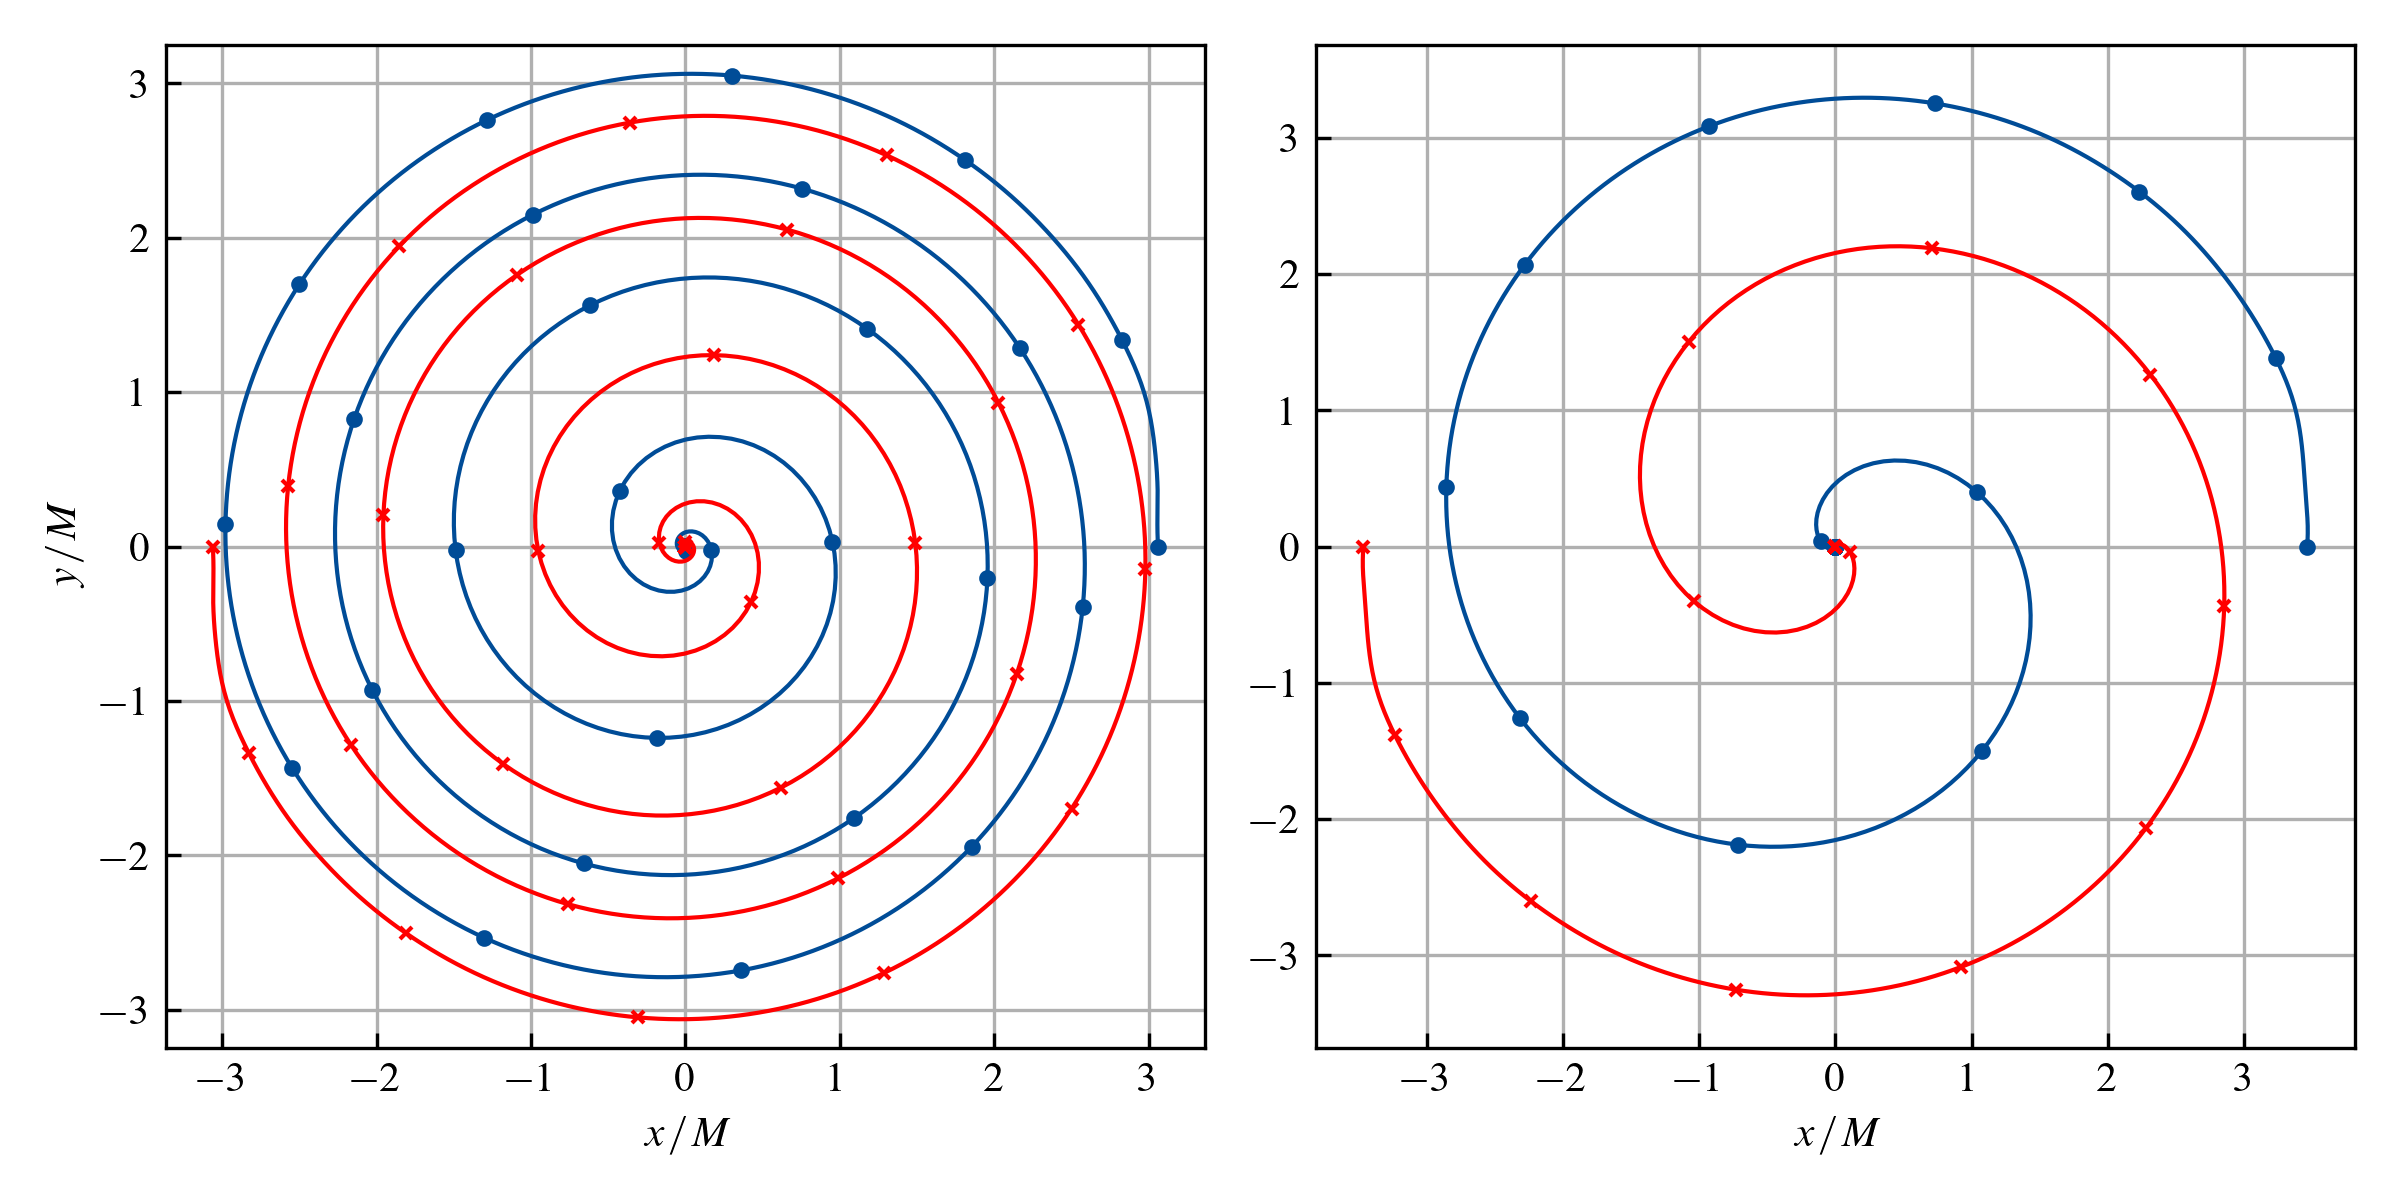
\includegraphics[width=\columnwidth]{img/traj}
		\caption{\label{fig:traj}The puncture trajectories on the $xy$ plane with ticks every $10.3186M$. Left shows the spin aligned case and right shows the spin antialigned case.}
	\end{figure}
	
	 
    \begin{figure}
      \centering
      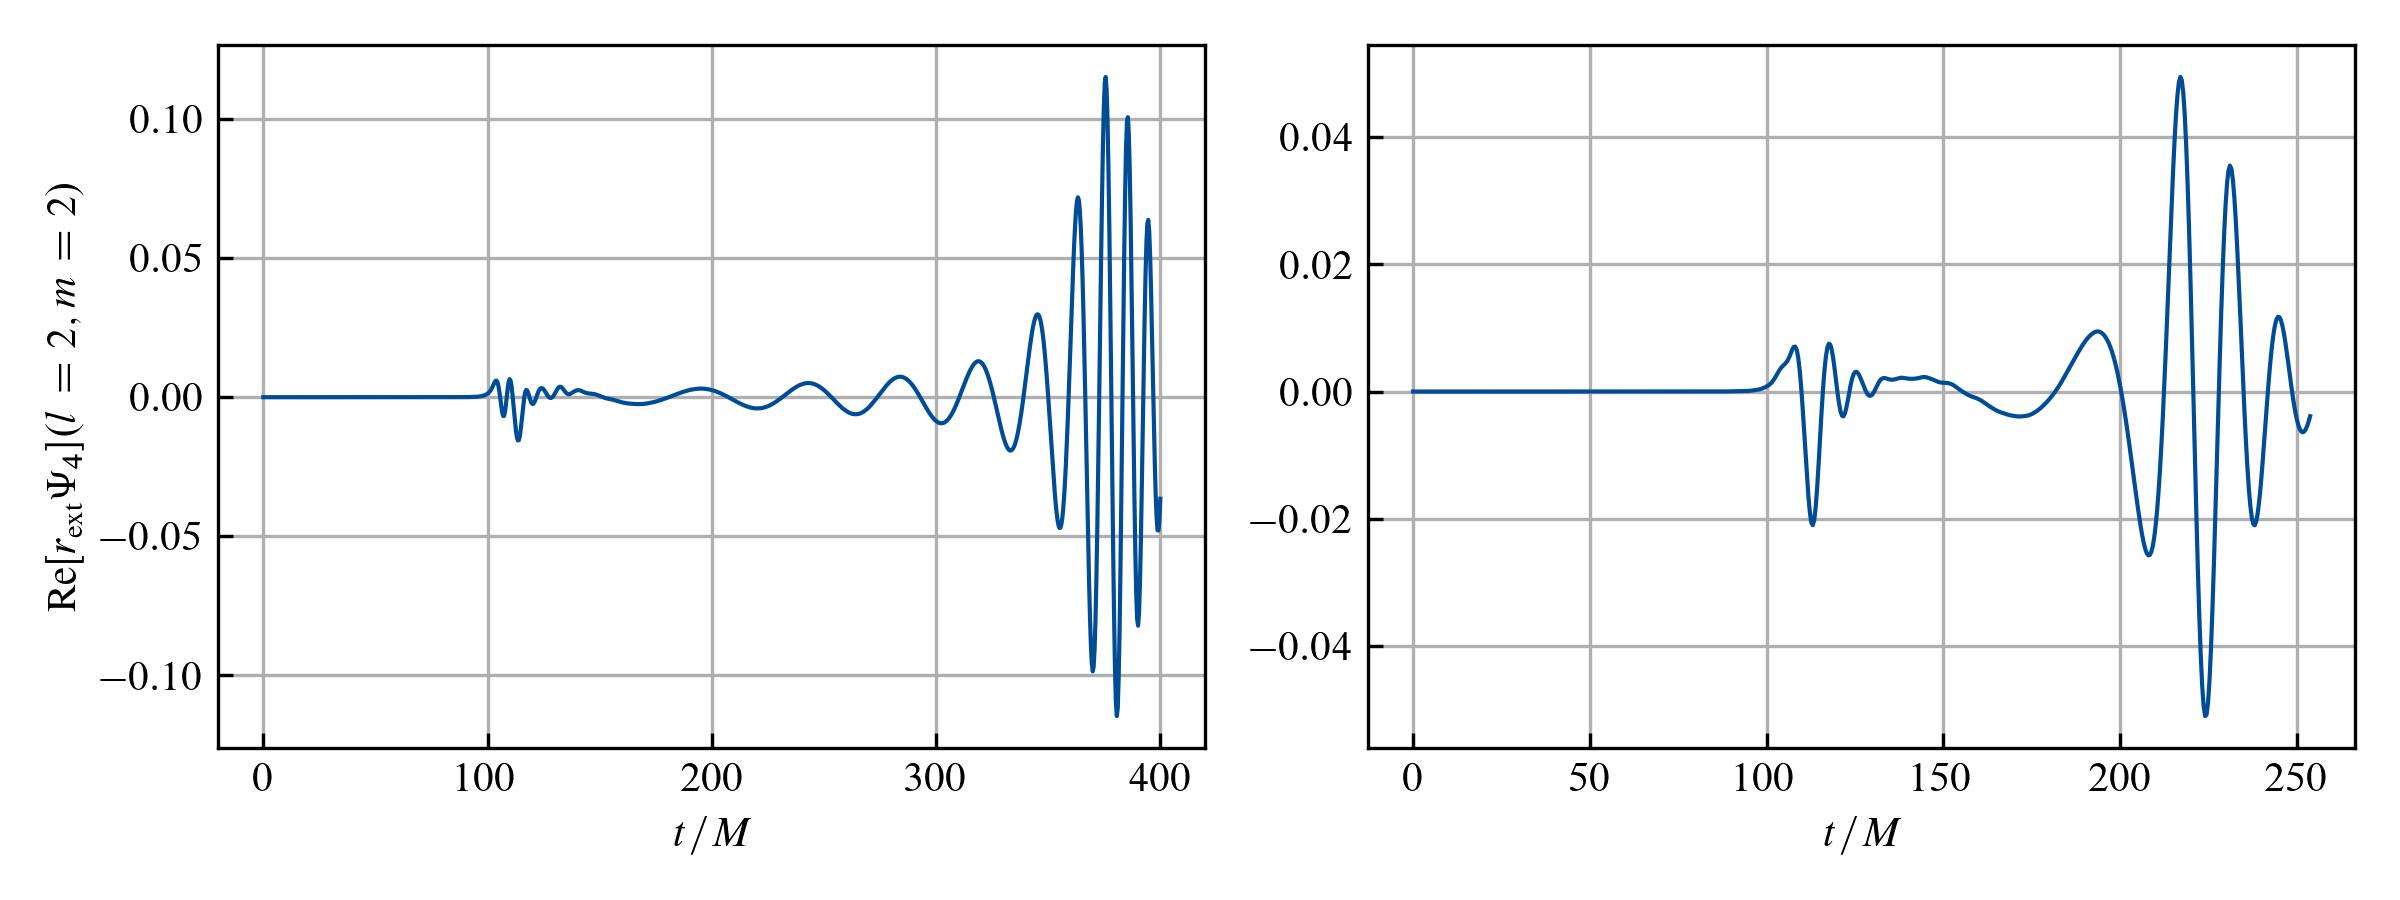
\includegraphics[width=\columnwidth]{img/Rerpsi4}
      \caption{\label{fig:rerpsi4}The real component of $r_\mathrm{ext}\psi_4$ at $r_\mathrm{ext}=100M$. Left shows the spin aligned case and right shows the spin antialigned case.}
    \end{figure}
    
    Figure~\ref{fig:psi4i} shows imaginary component of $\psi_4$ on $xz$ plane in aligned case. The first three images depict junk radiation, while the subsequent images show the actual gravitational wave emissions. Through this, we can confirm the intensity of gravitational waves based on the polar angle along the $z$-axis, clearly indicating that the intensity is greater closer to the $z$-axis.

  \end{block}


\end{column}

\separatorcolumn

\begin{column}{\colwidth}

  \begin{block}{}
  	
  	\begin{figure}
  		\centering
  		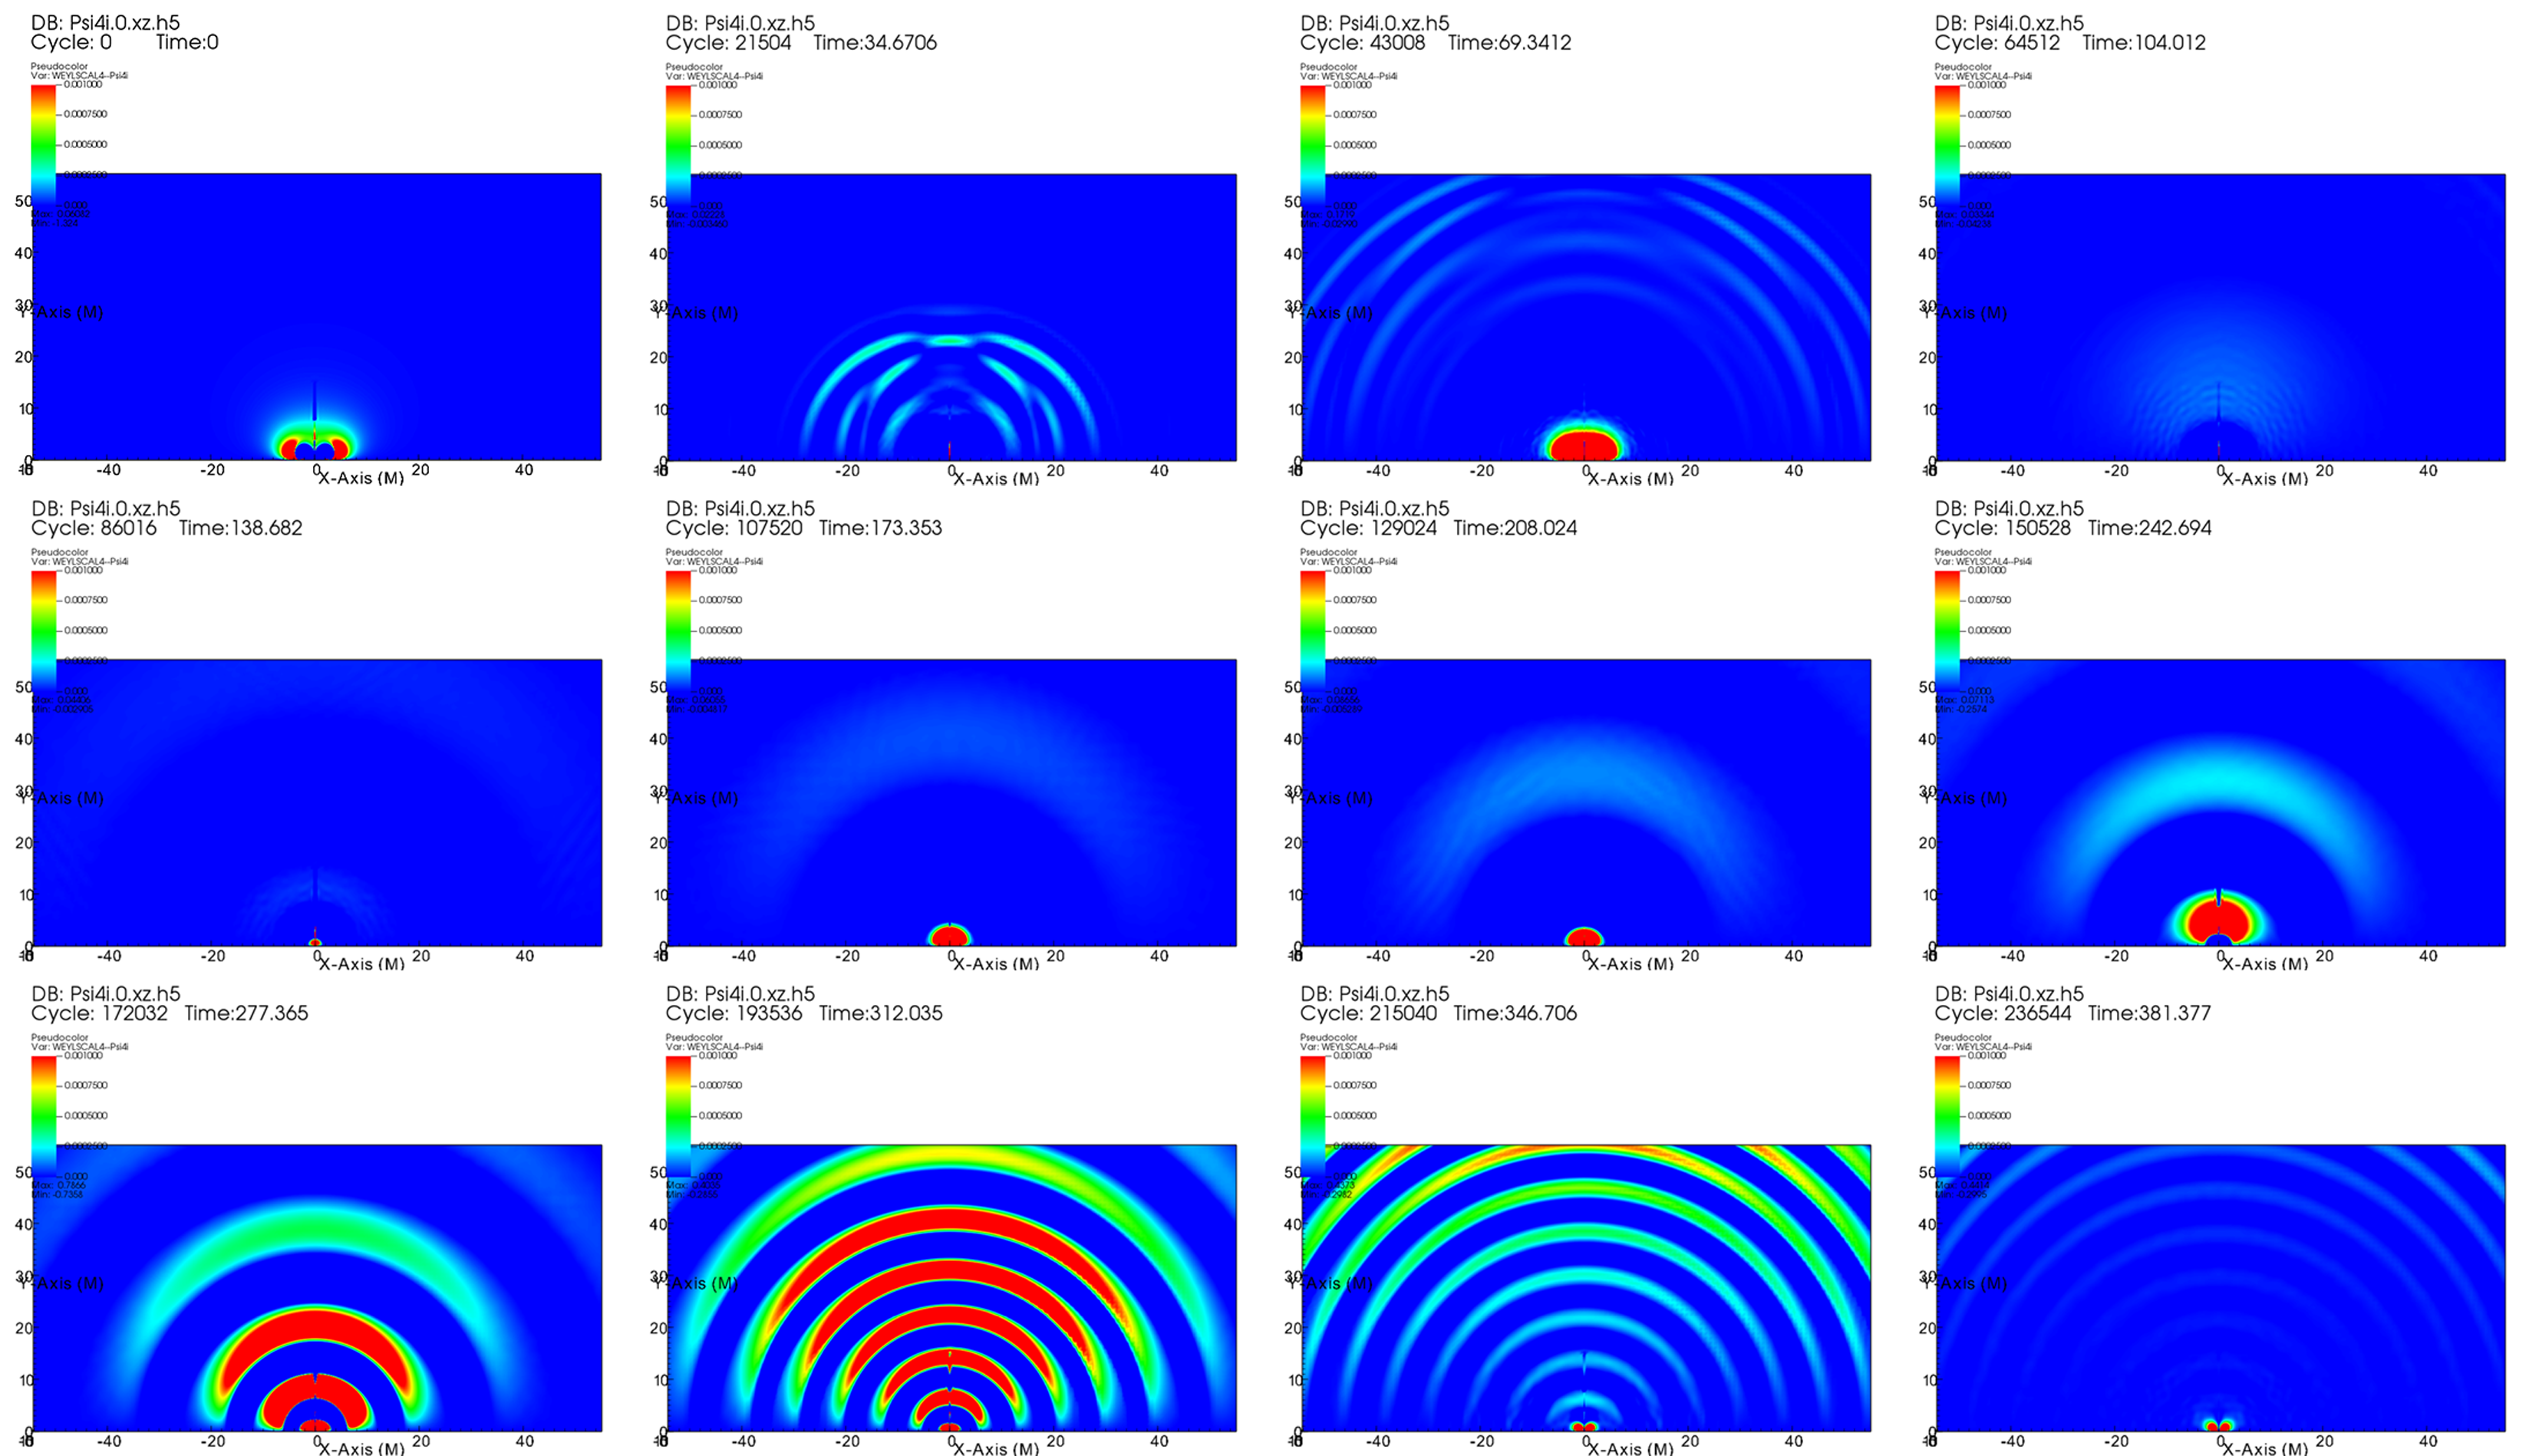
\includegraphics[width=\columnwidth]{img/psi4i}
  		\caption{\label{fig:psi4i}The imaginary component of $psi_4$ on $xz$ plane in aligned case. Each snapshot has a time interval of $34.6706M$.}
  	\end{figure}
	
	After the black hole merger, a Kerr black hole is left. The energy and angular momentum emitted through gravitational waves can be calculated by the difference in physical quantities of the Kerr black hole measured at the initial data and the end of the simulation. This value should match the value calculated through the following equation, as measured from $\psi_4$ as shown in Figure~\ref{fig:rerpsi4}:
	\begin{eqnarray}
		L_\mathrm{GW} = - \frac{dE}{dt} = \lim_{r\to\infty}{\frac{r^2}{16\pi}\sum_{l=2}^{\infty}\sum_{m=-l}^{l}\qty|\int_{-\infty}^{t}dt'\psi_4^{lm}|^2},
	\end{eqnarray}
	\begin{eqnarray}
		\frac{dJ_z}{dt}&=&\lim_{r\to\infty} \frac{r^2}{16\pi}\sum_{l=2}^{\infty}\sum_{m=-l}^{l}m \Im \biggl[\biggl(\int_{-\infty}^{t}dt'\psi_4^{lm}\biggr) \nonumber\\ &&\times \biggr( \int_{-\infty}^tdt'\int_{-\infty}^{t'}dt''\psi_4^{lm\ast} \biggr)\biggr].
	\end{eqnarray}
	Figure~\ref{fig:erad} and Figure~\ref{fig:jrad} depict $L_\mathrm{GW}$, $dJ_z/dt$, and their integrated values $E_\mathrm{rad}$ and $J_\mathrm{rad}$. Table~\ref{tab:comp} shows the values comparing each of them.
	\begin{figure}
		\centering
		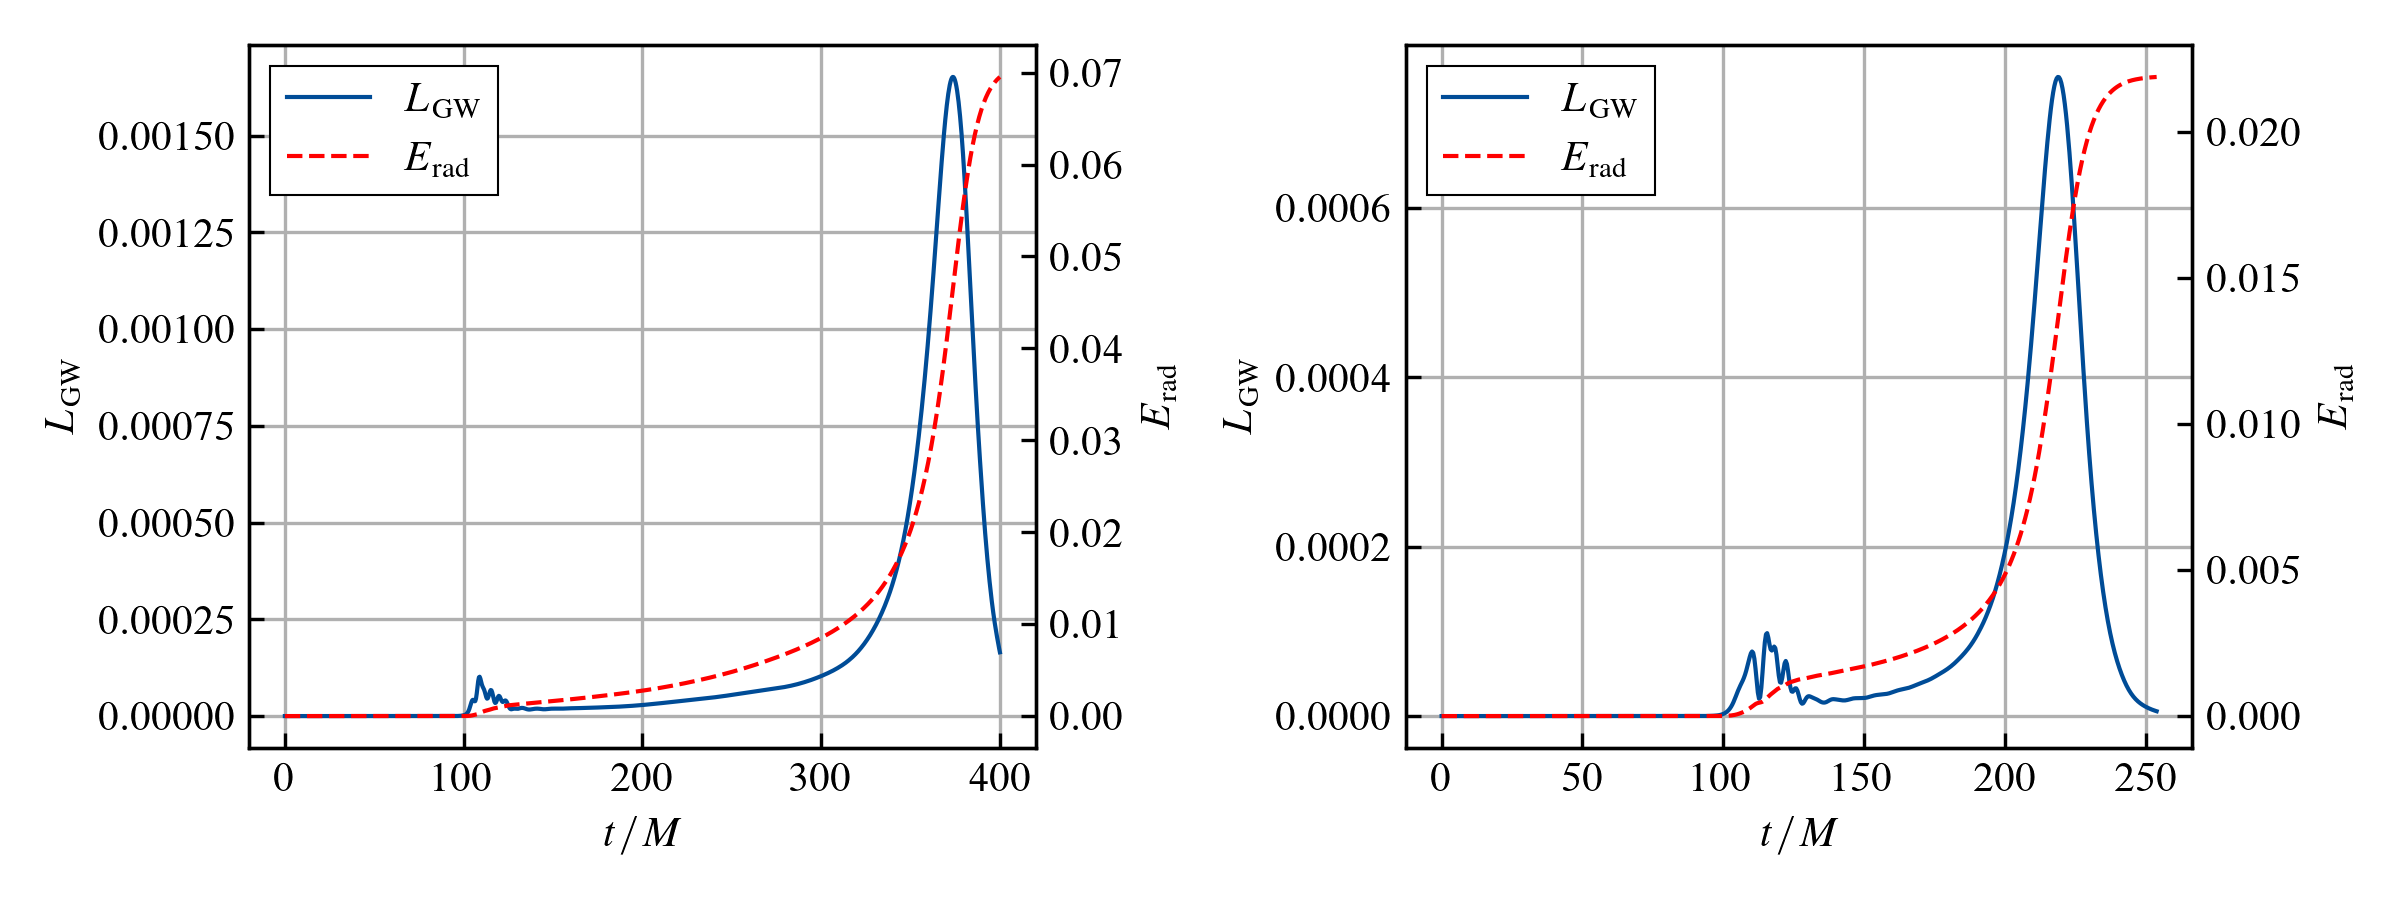
\includegraphics[width=\columnwidth]{img/erad}
		\caption{\label{fig:erad}The luminosity and accumulated radiated energy. Left shows the spin aligned case and right shows the spin antialigned case.}
	\end{figure}
	
	\begin{figure}
		\centering
		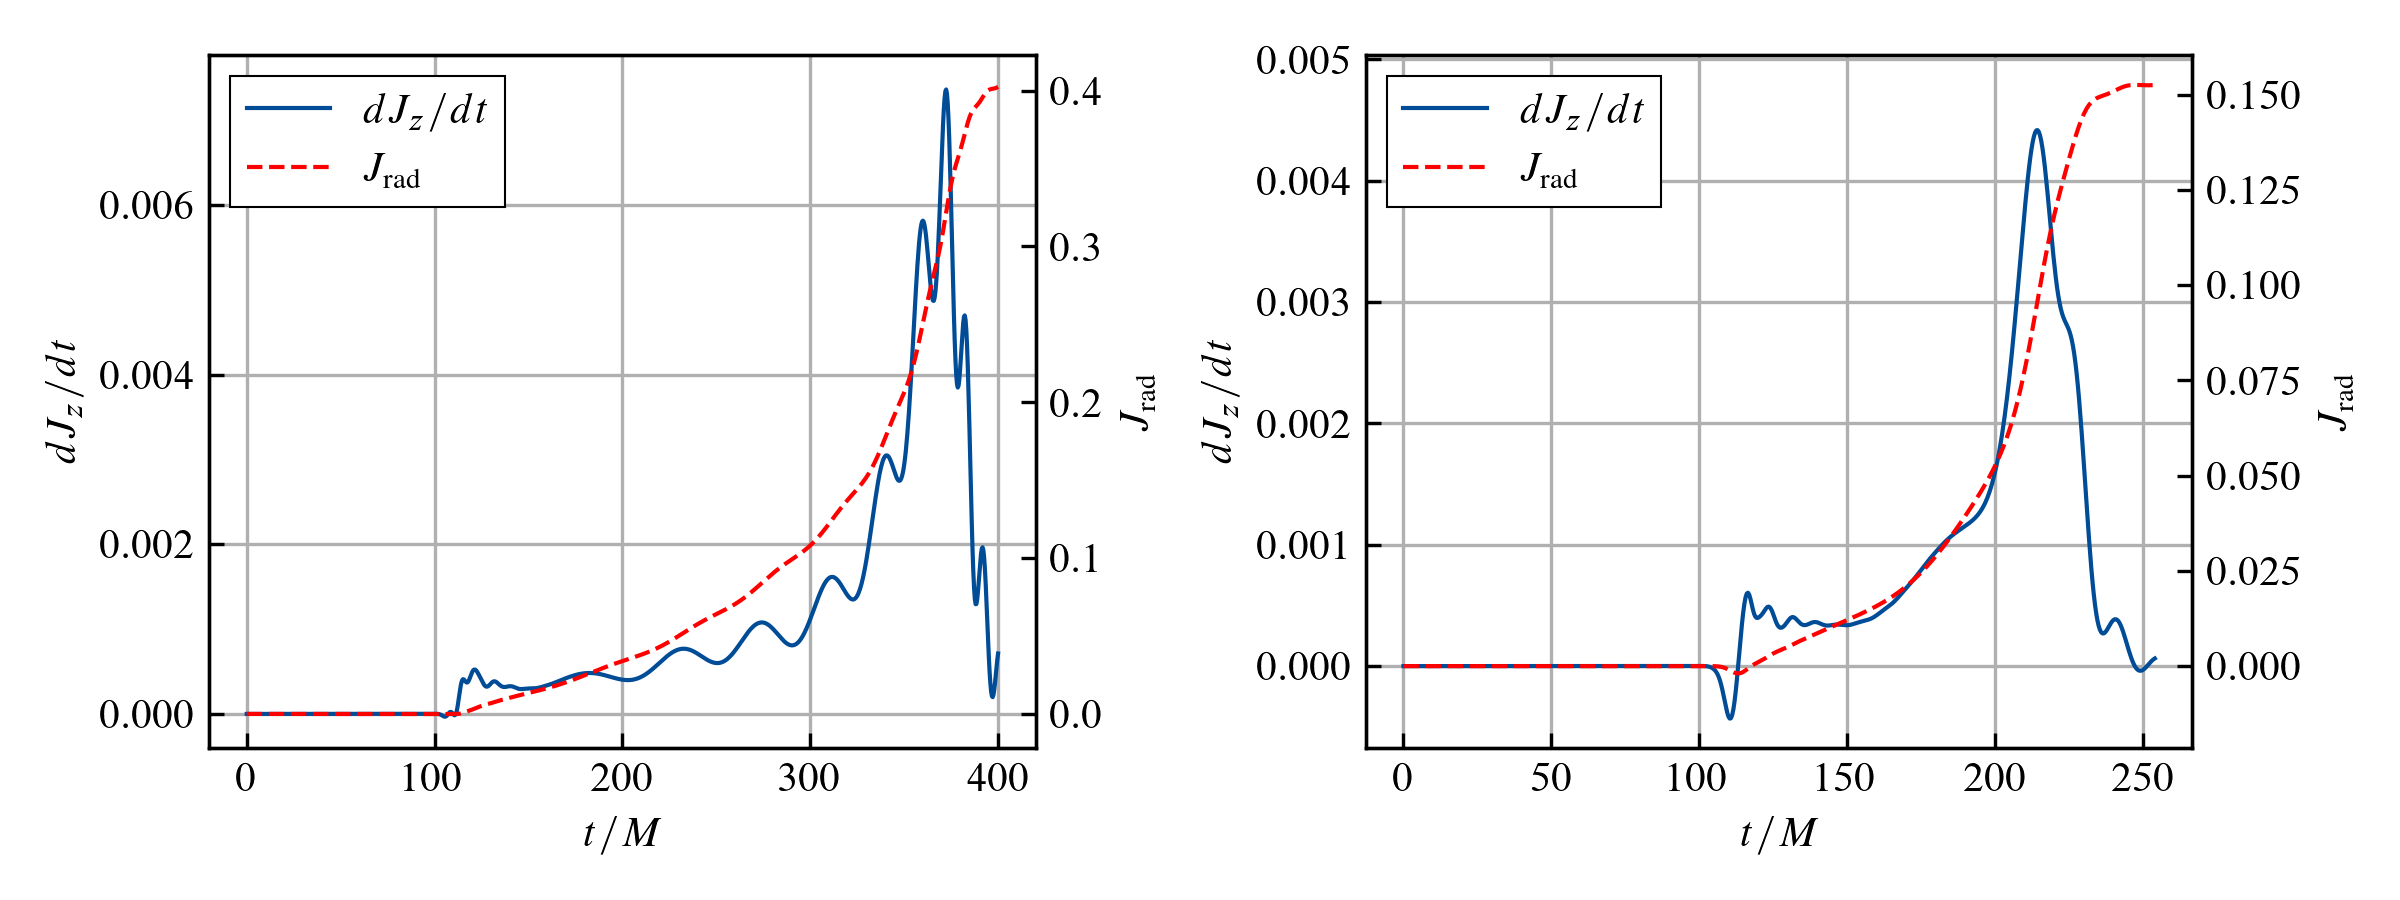
\includegraphics[width=\columnwidth]{img/jrad}
		\caption{\label{fig:jrad}The loss of angular momentum. Left shows the spin aligned case and right shows the spin antialigned case.}
	\end{figure}
	
	\begin{table}
		\centering
		\begin{tabular}{c c c}
			\toprule
			\textbf{} & \textbf{Aligned} & \textbf{Antialigned}\\
			\midrule
			$E_\mathrm{rad}^{(0)}/M_\mathrm{ADM}$ & 6.92\% & 2.16\% \\
			$E_\mathrm{rad}^{(1)}/M_\mathrm{ADM}$ & 6.95\% & 2.19\% \\
			$J_\mathrm{rad}^{(0)}/J_\mathrm{ADM}$ & 29.1\% & 24.7\% \\
			$J_\mathrm{rad}^{(1)}/J_\mathrm{ADM}$ & 34.1\% & 26.6\% \\
			\bottomrule
		\end{tabular}
		\caption{\label{tab:comp} The emitted energy and angular momentum are expressed as percentiles of the initial values. The superscript $(0)$ represents values calculated from metric information, and $(1)$ represents values calculated through gravitational waveforms.}
	\end{table}
	


  \end{block}

  \begin{block}{Conclusion}
	
    In this study, successful numerical simulations of spinning binary black holes were conducted. It was observed that the merger is delayed when the spins of both black holes are aligned in the same direction as the orbital angular momentum, compared to when they are antialigned. Furthermore, it was confirmed that a single Kerr black hole forms after the merger, and the spin is less than 1.
    
    In the next study, we will explore the impact of other physical quantities besides spin and investigate methods for initial data setup when spin is very high.

  \end{block}

  \begin{block}{References}

    \footnotesize{\bibliographystyle{plain}\bibliography{eintk}}

  \end{block}

\end{column}

\separatorcolumn
\end{columns}
\end{frame}

\end{document}
